\documentclass[
preprint, linenumbers,
% reprint,
% superscriptaddress,
% groupedaddress,
% unsortedaddress,
% runinaddress,
% frontmatterverbose, 
% preprint,
% preprintnumbers,
% nofootinbib,
% nobibnotes,
% bibnotes,
amsmath, amssymb, aps, physrev,
% pra,
% prb,
% rmp,
% prstab,
% prstper,
% floatfix,
]{revtex4-2}

\usepackage{dcolumn} % Align table columns on decimal point
\usepackage[utf8]{inputenc}
\usepackage{color}
\usepackage{graphicx}
\usepackage{placeins}
\usepackage[margin=1in]{geometry}
\usepackage{appendix}
\usepackage{amsmath, amssymb, bm}
\usepackage{multirow}
\usepackage{xfrac}
\usepackage[colorlinks=true, linkcolor=blue, citecolor=blue]{hyperref}
\usepackage[nameinlink, capitalize]{cleveref}
\usepackage[font=footnotesize, labelfont=bf]{caption}
\usepackage{subcaption}
\usepackage[version=4]{mhchem}
\usepackage{bm}
\usepackage{comment}
\usepackage[T1]{fontenc}
\usepackage{anyfontsize}
%\usepackage{newtxtext, newtxmath}
\newcommand{\?}{\stackrel{?}{=}}
\usepackage{tablefootnote}
\usepackage{stackengine}
\usepackage{mathrsfs} % For fancy \mathscr{S}
\usepackage{booktabs}
\usepackage{siunitx}
\sisetup{
 scientific-notation = true,
 round-mode = figures,
 round-precision = 3,
 table-number-alignment = center,
 retain-explicit-plus
}

\begin{document}

\preprint{Physical Review Letters}

\title{The contribution of nitrogen Frenkel-pair formation to the high-temperature heat capacity of uranium mononitride}
% On the role of nitrogen Frenkel-pair formation in the high-temperature heat capacity of uranium mononitride

% Nitrogen sublattice disorder as a candidate mechanism for excess heat capacity in uranium mononitride

\author{Mohamed AbdulHameed$^{1}$}
\author{Benjamin Beeler$^{1,2}$\thanks{Corresponding author: \href{mailto:bwbeeler@ncsu.edu}{bwbeeler@ncsu.edu}}}

\affiliation{$^{1}$Department of Nuclear Engineering, North Carolina State University, Raleigh, NC 27695}
\affiliation{$^{2}$Idaho National Laboratory, Idaho Falls, ID 83415}

\date{\today}

\begin{abstract}
The high-temperature heat capacity of uranium mononitride (UN) remains uncertain due to conflicting measurements and models above $\sim$1700~K. To assess whether intrinsic defect formation contributes to the observed superlinear behavior of $C_P(T)$, we perform large-scale molecular dynamics simulations using two interatomic potentials to quantify nitrogen diffusion and Frenkel-pair populations from 1800--2600~K. Both models show increasing anion mobility, but the Tseplyaev potential yields substantially larger Frenkel concentrations, producing a defect heat-capacity contribution of up to $\sim$10~J/(mol-K). This defect-driven term is consistent with the curvature seen in historical correlations and recent \textit{ab initio} results, suggesting that nitrogen sublattice disorder provides a plausible intrinsic mechanism for the high-temperature heat capacity of UN. % High-purity experiments are needed to confirm its magnitude.
\end{abstract}

\maketitle

The specific heat, $C_P$, of uranium mononitride (UN) is not yet conclusively established, with experimental datasets and theoretical predictions offering conflicting descriptions above roughly 1700~K. The most widely used correlation, developed by Hayes \textit{et al.}~\cite{Hayes1990IV}, exhibits a strongly superlinear increase in $C_P(T)$ at elevated temperatures, approaching a nearly $T^{5}$ dependence~\cite{AbdulHameed2024}. This trend originates from the high–temperature enthalpy measurements of Conway and Flagella~\cite{Conway1969}, which extend to approximately 2600~K and remain the only measurements reaching such elevated temperatures. The only other available high–temperature measurements, i.e., those by Affortit~\cite{Affortit1970} that extend up to about 2300~K, report an almost linear temperature dependence. They also report higher $C_P(T)$ values than all other datasets in the temperature range of 1200--1900~K. Thus, Hayes \textit{et al.}~\cite{Hayes1990IV} decided to disregard Affortit's dataset and rely only on the measurements of Conway and Flagella to extract $C_P(T)$ at high temperatures. % Note that both the Conway-Flagella and Affortit studies used calorimetry, with Conway and Flagella measuring the enthalpy and Affortit measuring the specific heat directly.

A central complication arises from the composition of the Conway-Flagella samples, which contained roughly 20~wt.\% UO$_2$. Because UO$_2$ exhibits a premelting (superionic) transition driven by oxygen Frenkel defects~\cite{Pavlov2017,Cooper2014}, any attempt to extract a UN-specific enthalpy from mixed-material calorimetry requires subtracting a defect-rich UO$_2$ contribution whose behavior changes rapidly with temperature \cite{Hayes1990IV}. While the specific heat capacity extracted from Conway-Flagella enthalpy measurements agrees with other datasets at moderate temperature \cite{Hayes1990IV}, it develops a strong upward curvature when extrapolated above $\sim$1700~K. Given the known defect thermodynamics of UO$_2$ \cite{Pavlov2017,Cooper2014}, this trend could plausibly reflect the UO$_2$ component rather than the intrinsic response of UN \cite{Galvin2023}.

Theoretical predictions also diverge. Early \textit{ab initio} molecular dynamics (AIMD) simulations reported an nearly perfectly linear $C_{P}(T)$~\cite{Kocevski2023}. Classical molecular dynamics (MD) using the angular-dependent potential (ADP) of Tseplyaev and Starikov~\cite{Kuksin2016,Tseplyaev2016} reproduced a steep increase in $C_P(T)$ consistent with the Hayes correlation~\cite{AbdulHameed2024}. The embedded atom method (EAM) potential of Kocevski \textit{et al.}~\cite{Kocevski2022II} also predicts a nearly linear $C_P(T)$ at high temperatures \cite{AbdulHameed2024}. Recent AIMD simulations combined with the disorded local moment (DLM) method predict a $T^{2}$-like increase in $C_P(T)$~\cite{AbdulHameed2025}. This result is significant because AIMD+DLM is a first-principles method that treats both lattice dynamics and magnetic disorder on equal footing. The fact that a high-accuracy \textit{ab initio} calculation yields a moderate, $T^{2}$-like increase suggests that while the anomaly is likely less dramatic than the historical correlation implies, there is independent evidence that a nonlinear increase in $C_{P}(T)$ is an intrinsic feature of UN at high temperatures.

The unresolved question is not only the magnitude of the heat capacity but the physical origin of its temperature dependence. Galvin \textit{et al.} \cite{Galvin2023} argued that current data support two plausible interpretations: either the Kocevski potential correctly predicts an asymptotically linear high-temperature heat capacity and the Conway-Flagella curvature is extrinsic, likely influenced by UO$_2$ in the samples, or the stronger rise seen with the Tseplyaev potential reflects an intrinsic mechanism in UN that has not yet been experimentally confirmed. They also suggested that strong anharmonicity, phonon softening, or even partial UN decomposition could contribute to the observed rise in $C_P(T)$ if defect mechanisms alone are insufficient.

A useful reference is the defect thermodynamics of UO$_2$, where oxygen Frenkel pairs proliferate as the temperature approaches the superionic transition, producing large excess contributions to both enthalpy and heat capacity~\cite{Pavlov2017}. MD simulations by Cooper \textit{et al.}~\cite{Cooper2014} demonstrated that oxygen diffusion increases sharply and $C_{P}(T)$ exhibits a broad anomaly near 2700~K as the anion sublattice disorders. Because Conway–Flagella's samples contained enough UO$_2$ to contribute significantly to the measured enthalpy, it is plausible that the reconstructed UN correlation inherited part of this defect-driven curvature. However, the nonlinear $T^{2}$-like behavior obtained in recent AIMD+DLM simulations~\cite{AbdulHameed2025} suggests that a degree of intrinsic anion–sublattice softening may also occur in UN. This raises the question whether nitrogen Frenkel-pair formation in UN could contribute to UN's $C_P(T)$ analogous to that observed in UO$_2$.

To address this question, we performed classical MD simulations of UN using two interatomic potentials: the Tseplyaev angular-dependent potential \cite{Tseplyaev2016} and the Kocevski EAM potential. All calculations eutilize the Large-scale Atomic/Molecular Massively Parallel Simulator (LAMMPS) software package \cite{Plimpton1995, Thompson2022} using a 1 fs time step, with periodic boundary conditions (PBCs) applied in all directions. The OVITO software package \cite{Stukowski2010} is used for supercell visualization and analysis. All simulations employ a $50 \times 50 \times 50$ supercell ($10^6$ atoms), allowing us to sample both transport and point-defect statistics over the  temperature range of 1800--2600~K. For diffusivity calculations, the supercells are equilibrated in the \textit{NPT} ensemble and then evolved for a total of 5~ns. The self-diffusion coefficients are obtained from the long-time limit of the mean-squared displacement, MSD,
\begin{equation}
D = \lim_{t\rightarrow\infty}\frac{\langle \Delta r^{2}(t) \rangle}{6t},
\end{equation}
using the slope over the final 3~ns of each trajectory. No defects were inserted in any of these simulations, and all contributions to the MSD originate from spontaneously produced Frenkel pairs. In all cases, uranium remained effectively immobile on these timescales, while nitrogen exhibited increasingly rapid motion with temperature.

\begin{figure*}[h!]
\centering
\begin{subfigure}{0.45\textwidth}
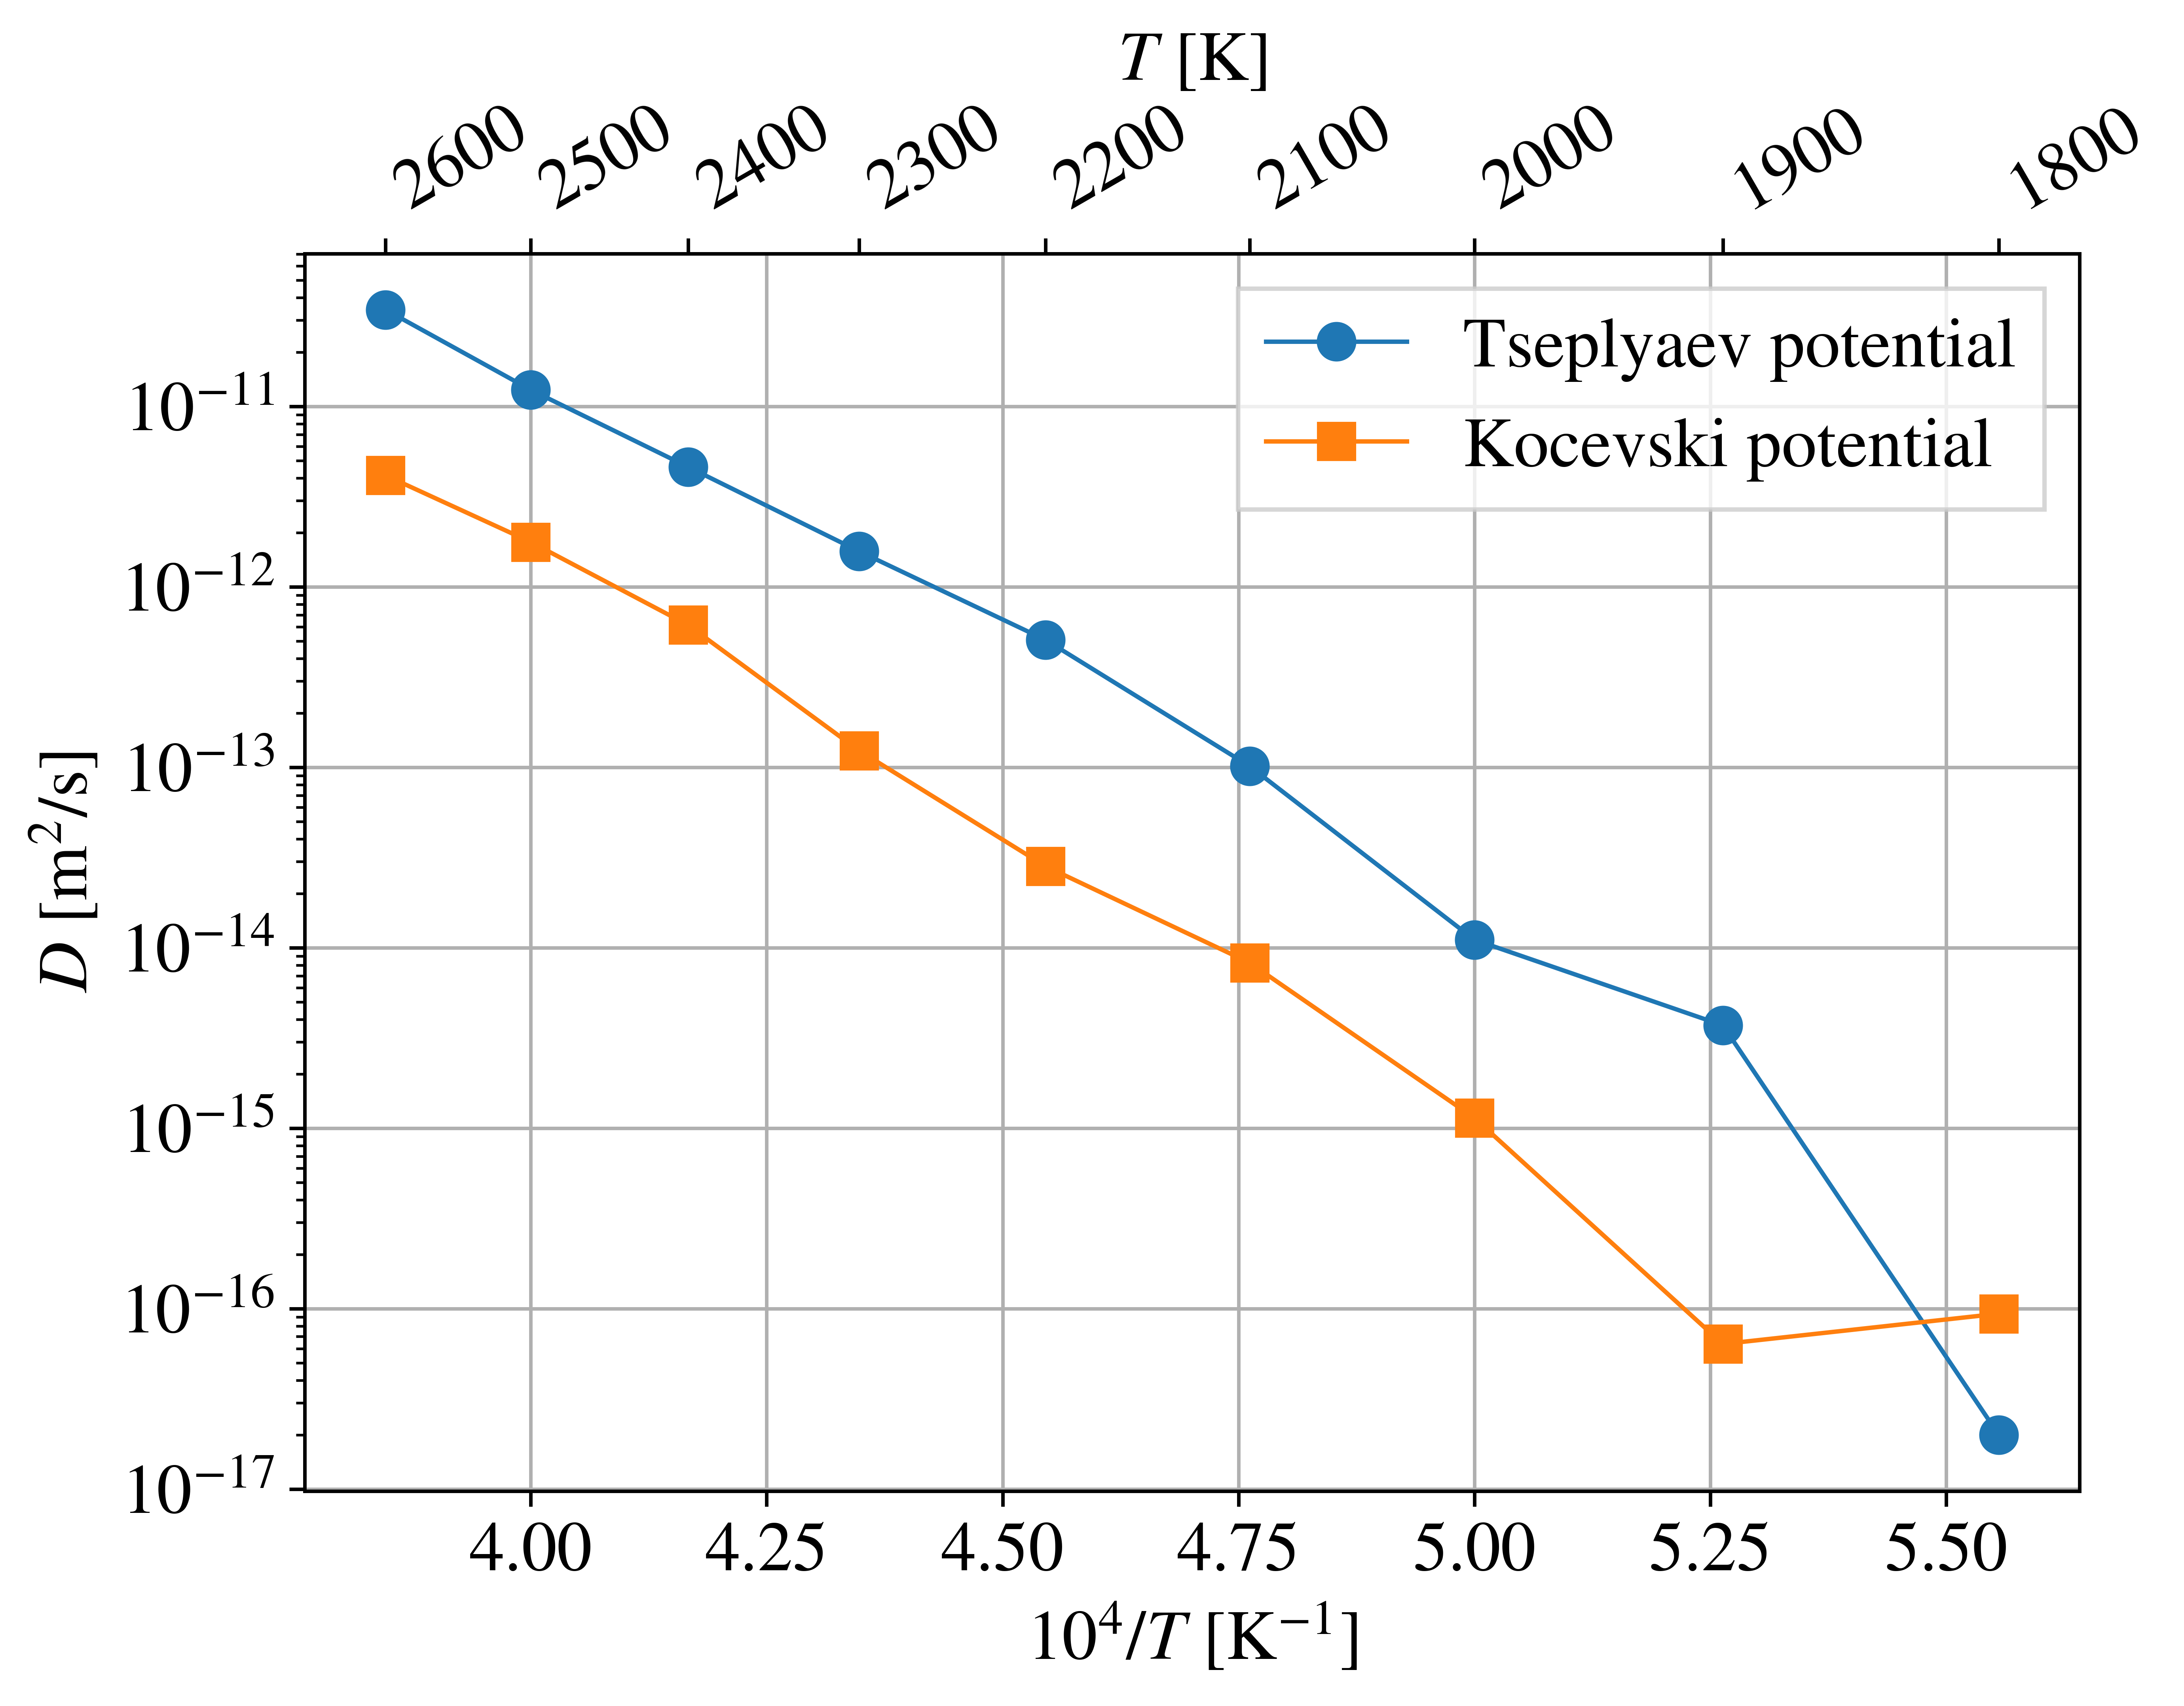
\includegraphics[width=\textwidth]{DN.png}
\caption{}
\label{Fig:D}
\end{subfigure}
\hfill
\begin{subfigure}{0.45\textwidth}
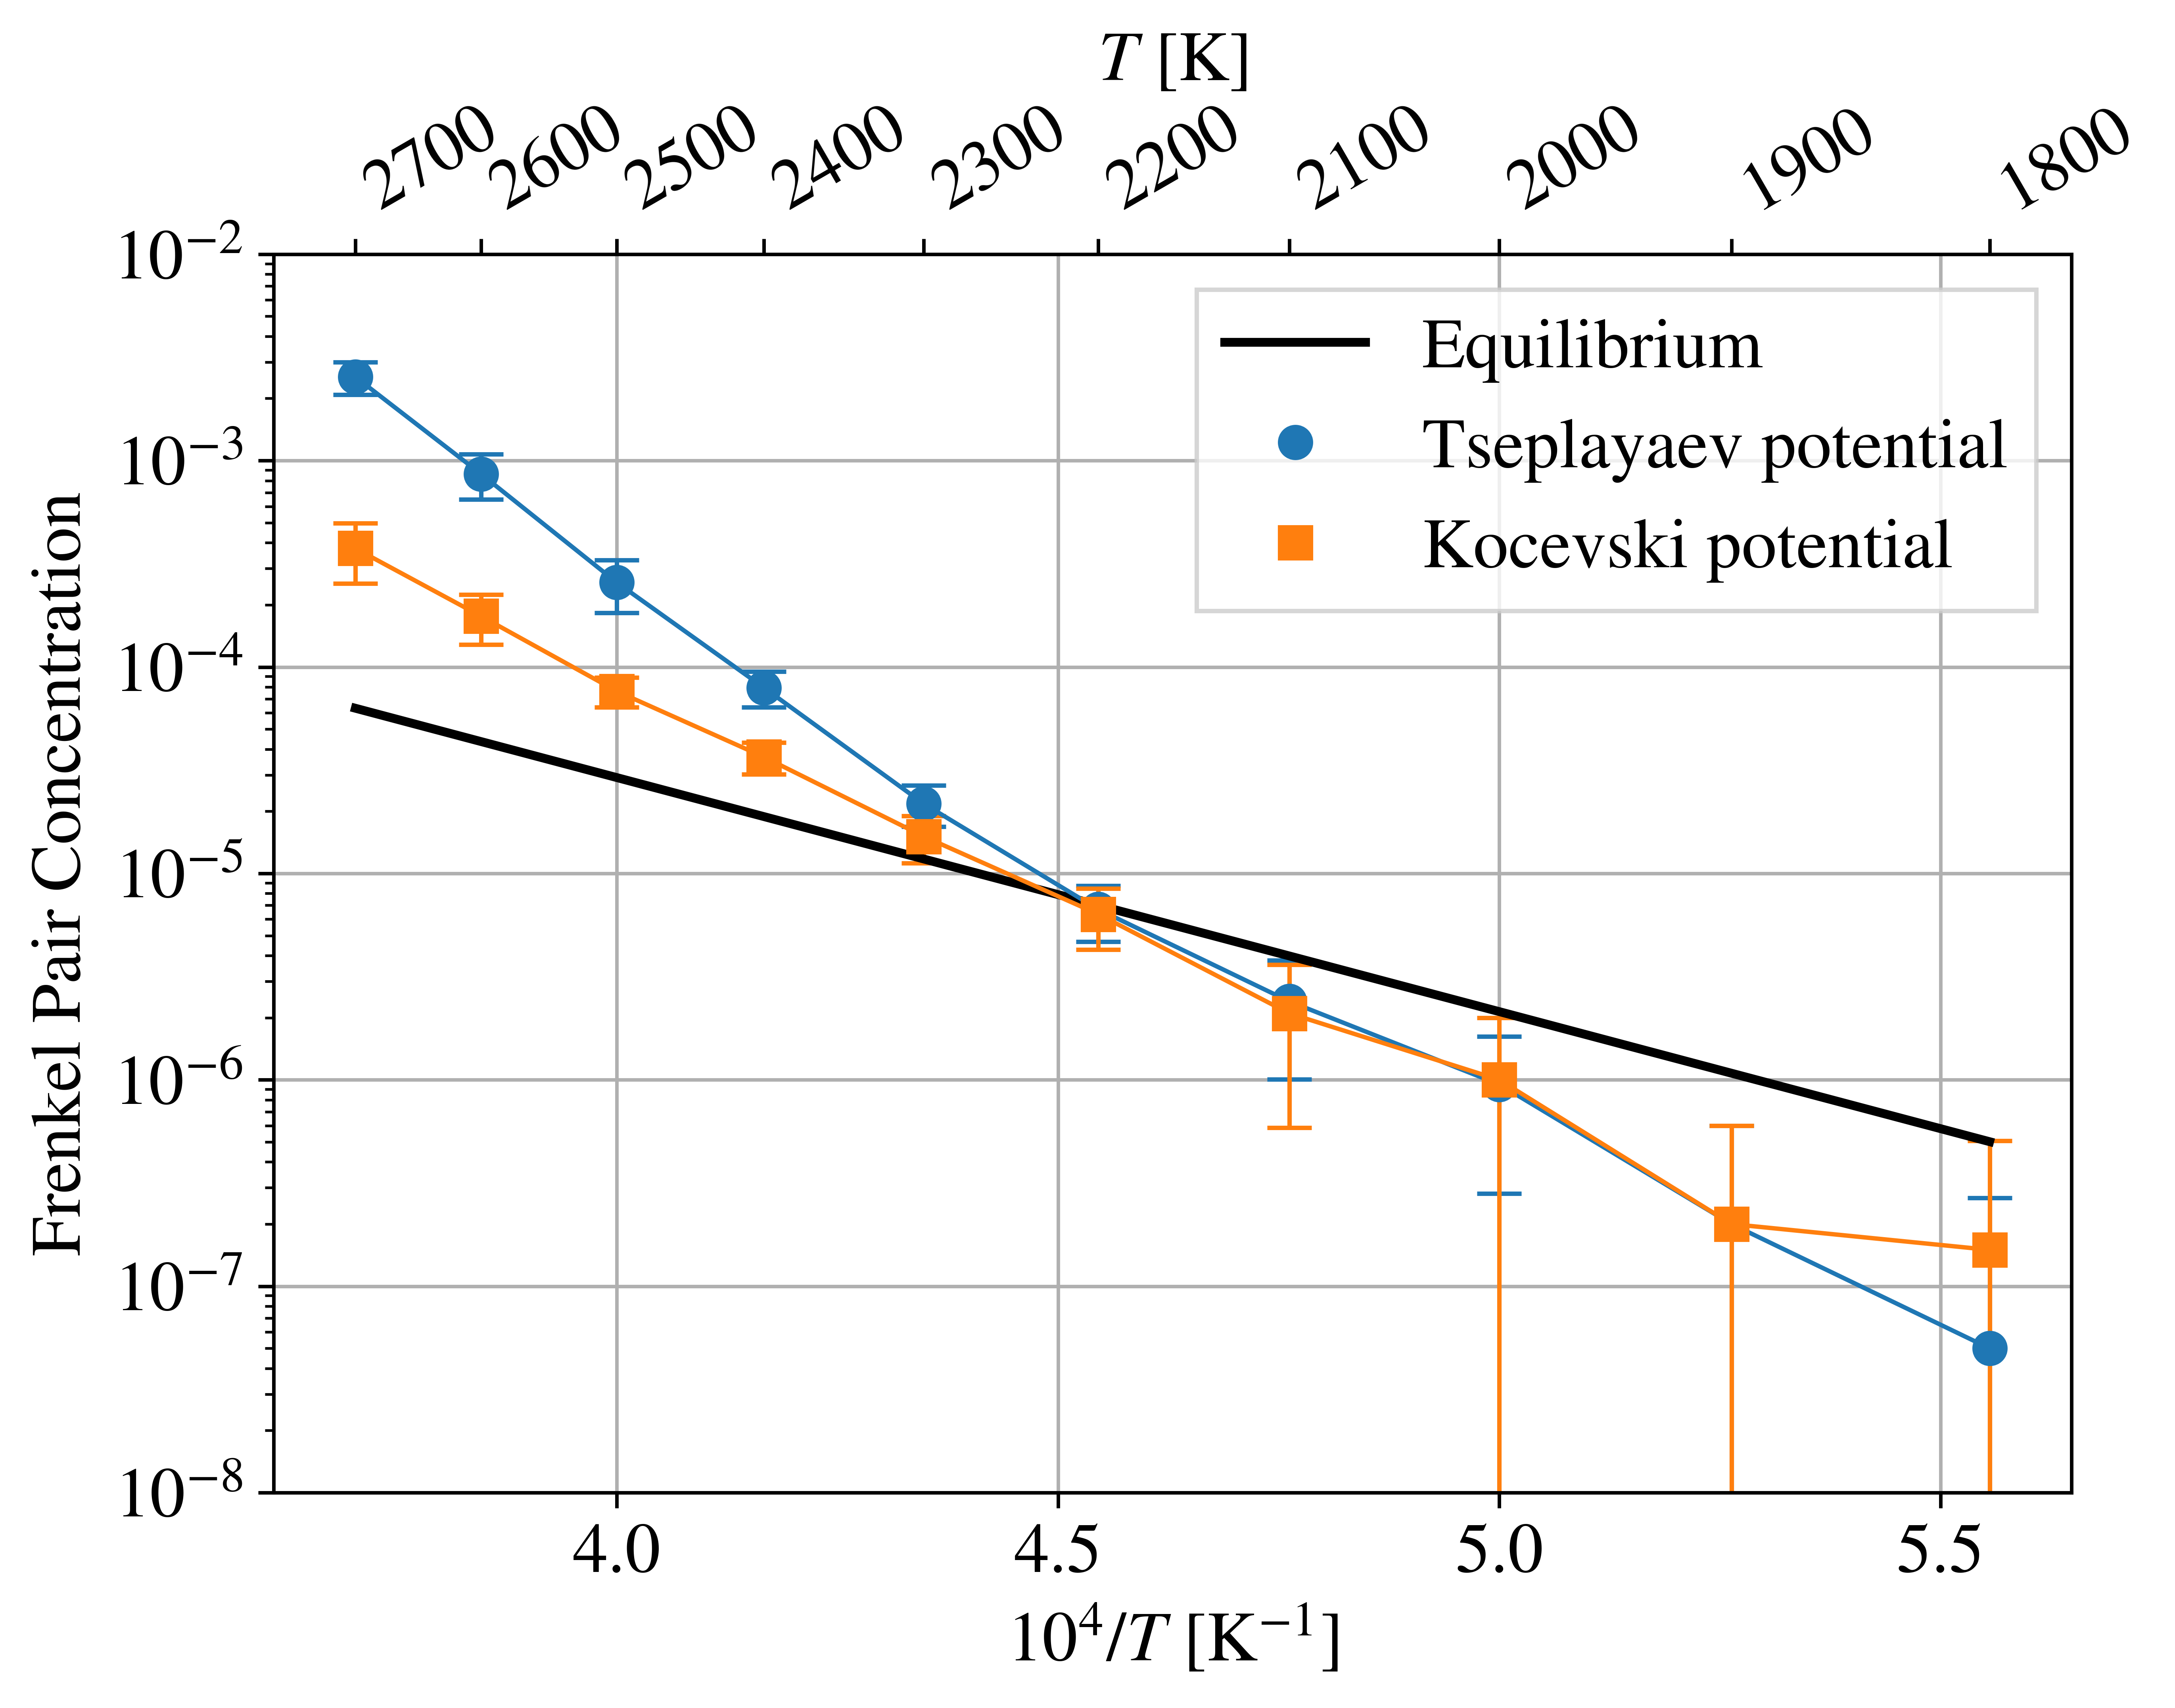
\includegraphics[width=\textwidth]{FrenkelConc.png}
\caption{}
\label{Fig:C}
\end{subfigure}
\caption{(Color online) (\textbf{a}) Nitrogen self-diffusion coefficients obtained from MSD analysis. (\textbf{b}) Nitrogen Frenkel-pair concentrations extracted using Wigner–Seitz defect analysis over 200~ps trajectories. Data points denote temporal averages over the post-equilibration sampling window, and error bars represent the standard deviation obtained from time averaging. The equilibrium concentration is based on Frenkel-pair formation energy of 4.5 eV calculated elsewhere using DFT and 0 K MD \cite{Yang2021,Kocevski2022I,AbdulHameed2024}.}
\end{figure*}

\cref{Fig:D} summarizes the nitrogen self-diffusion coefficients for both potentials. For the Tseplyaev potential, the nitrogen diffusivity, $D_\text{N}$, is essentially zero at temperatures below 1800~K and then increases sharply, rising from $3.7\times10^{-15}$~m$^{2}$/s at 1900~K to $3.4\times10^{-11}$~m$^{2}$/s at 2600~K, spanning nearly four orders of magnitude. The Kocevski potential yields the same qualitative trend but with systematically smaller values, typically one order of magnitude lower across the entire range, with $D_\text{N}$ approaching $4.1 \times 10^{-12}$~m$^{2}$/s at 2600~K. The increasing nitrogen transport above 1800--1900~K, especially for the Tseplyaev potential, coincides with the temperature range where the Conway-Flagella enthalpy data start deviating from an approximately linear trend into a pronounced nonlinear increase. This suggests that the same microscopic process responsible for the rapid growth of nitrogen mobility---namely, the onset of significant anion-sublattice disorder and Frenkel-pair formation---may also underlie the excess enthalpy that produces the apparent high-temperature anomaly in the empirical heat capacity.

To more directly quantify point-defect formation, we analyzed nitrogen Frenkel-pair concentrations using the Wigner-Seitz (WS) defect analysis implemented in OVITO \cite{Stukowski2010}. In this method, a defect-free reference lattice defines the positions of ideal sites, each associated with a Wigner-Seitz cell, i.e., the region of space closer to that site than to any other. For a given instantaneous configuration, each atom is assigned to the nearest reference site. Sites with occupancy zero correspond to vacancies, while sites with occupancy greater than one indicate interstitial defects. This nearest-site mapping provides a robust, topology-based identification of point defects. For each temperature, we simulated for 200~ps, recorded snapshots every 10~ps, and applied the WS analysis to all configurations after the first 10~ps to ensure equilibration. The reported Frenkel-pair concentrations correspond to the time-averaged mean over the sampled configurations, and the associated error bars represent the standard deviation over the temporal sampling window.

The resulting nitrogen Frenkel-pair concentrations, $c_{\mathrm{FP}}(T)$, are shown in \cref{Fig:C}. For the Tseplyaev potential, $c_{\mathrm{FP}}$ increases from $5\times10^{-8}$ at 1800~K to $8.6\times10^{-4}$ at 2600~K. Fitting an Arrhenius form,
\begin{equation}
c_{\mathrm{FP}}(T) \propto \exp\!\left[-\frac{Q}{k_{\mathrm{B}}T}\right],
\end{equation}
yields an effective activation energy $Q_{\mathrm{ADP}} = 4.97$~eV, while the Kocevski potential produces a lower activation energy, $Q_{\mathrm{EAM}} = 3.79$~eV, and lower defect populations at all temperatures. Thus, the Tseplyaev potential generates nitrogen Frenkel concentrations large enough to potentially alter the thermodynamics.

% not only reproduces DFT formation energies more faithfully, but it also 
% in good agreement with reported DFT and MD values for the nitrogen Frenkel pair formation energy ($4.5$--$5.0$~eV) \cite{Kocevski2022I,AbdulHameed2024}.

Frenkel-pair formation contributes an additional term to the heat capacity \cite{Szwarc1969,Pavlov2017}:
\begin{equation}
C_{\mathrm{def}}(T) = \frac{1}{n_{\mathrm{moles}}} \frac{\partial}{\partial T} \left[n_{\mathrm{FPs}}(T) \ Q \right]
\approx \frac{Q}{n_{\mathrm{moles}}} \frac{\partial n_{\mathrm{FPs}}}{\partial T}.
\label{Eq:C_def}
\end{equation}
In practice, we evaluate $C_{\mathrm{def}}(T)$ directly from the Frenkel-pair populations obtained by the WS analysis for both interatomic potentials. We assume a formation enthalpy $Q$ = 4.5~eV, consistent with both the DFT estimates \cite{Yang2021,Kocevski2022I} and the $T \rightarrow 0$~K Frenkel pair formation energies of both the Tseplyaev and Kocevski potentials~\cite{AbdulHameed2024}. The temperature derivative in \cref{Eq:C_def} is computed using centered finite differences applied to the simulated defect populations.

\begin{figure*}[h!]
 \centering
 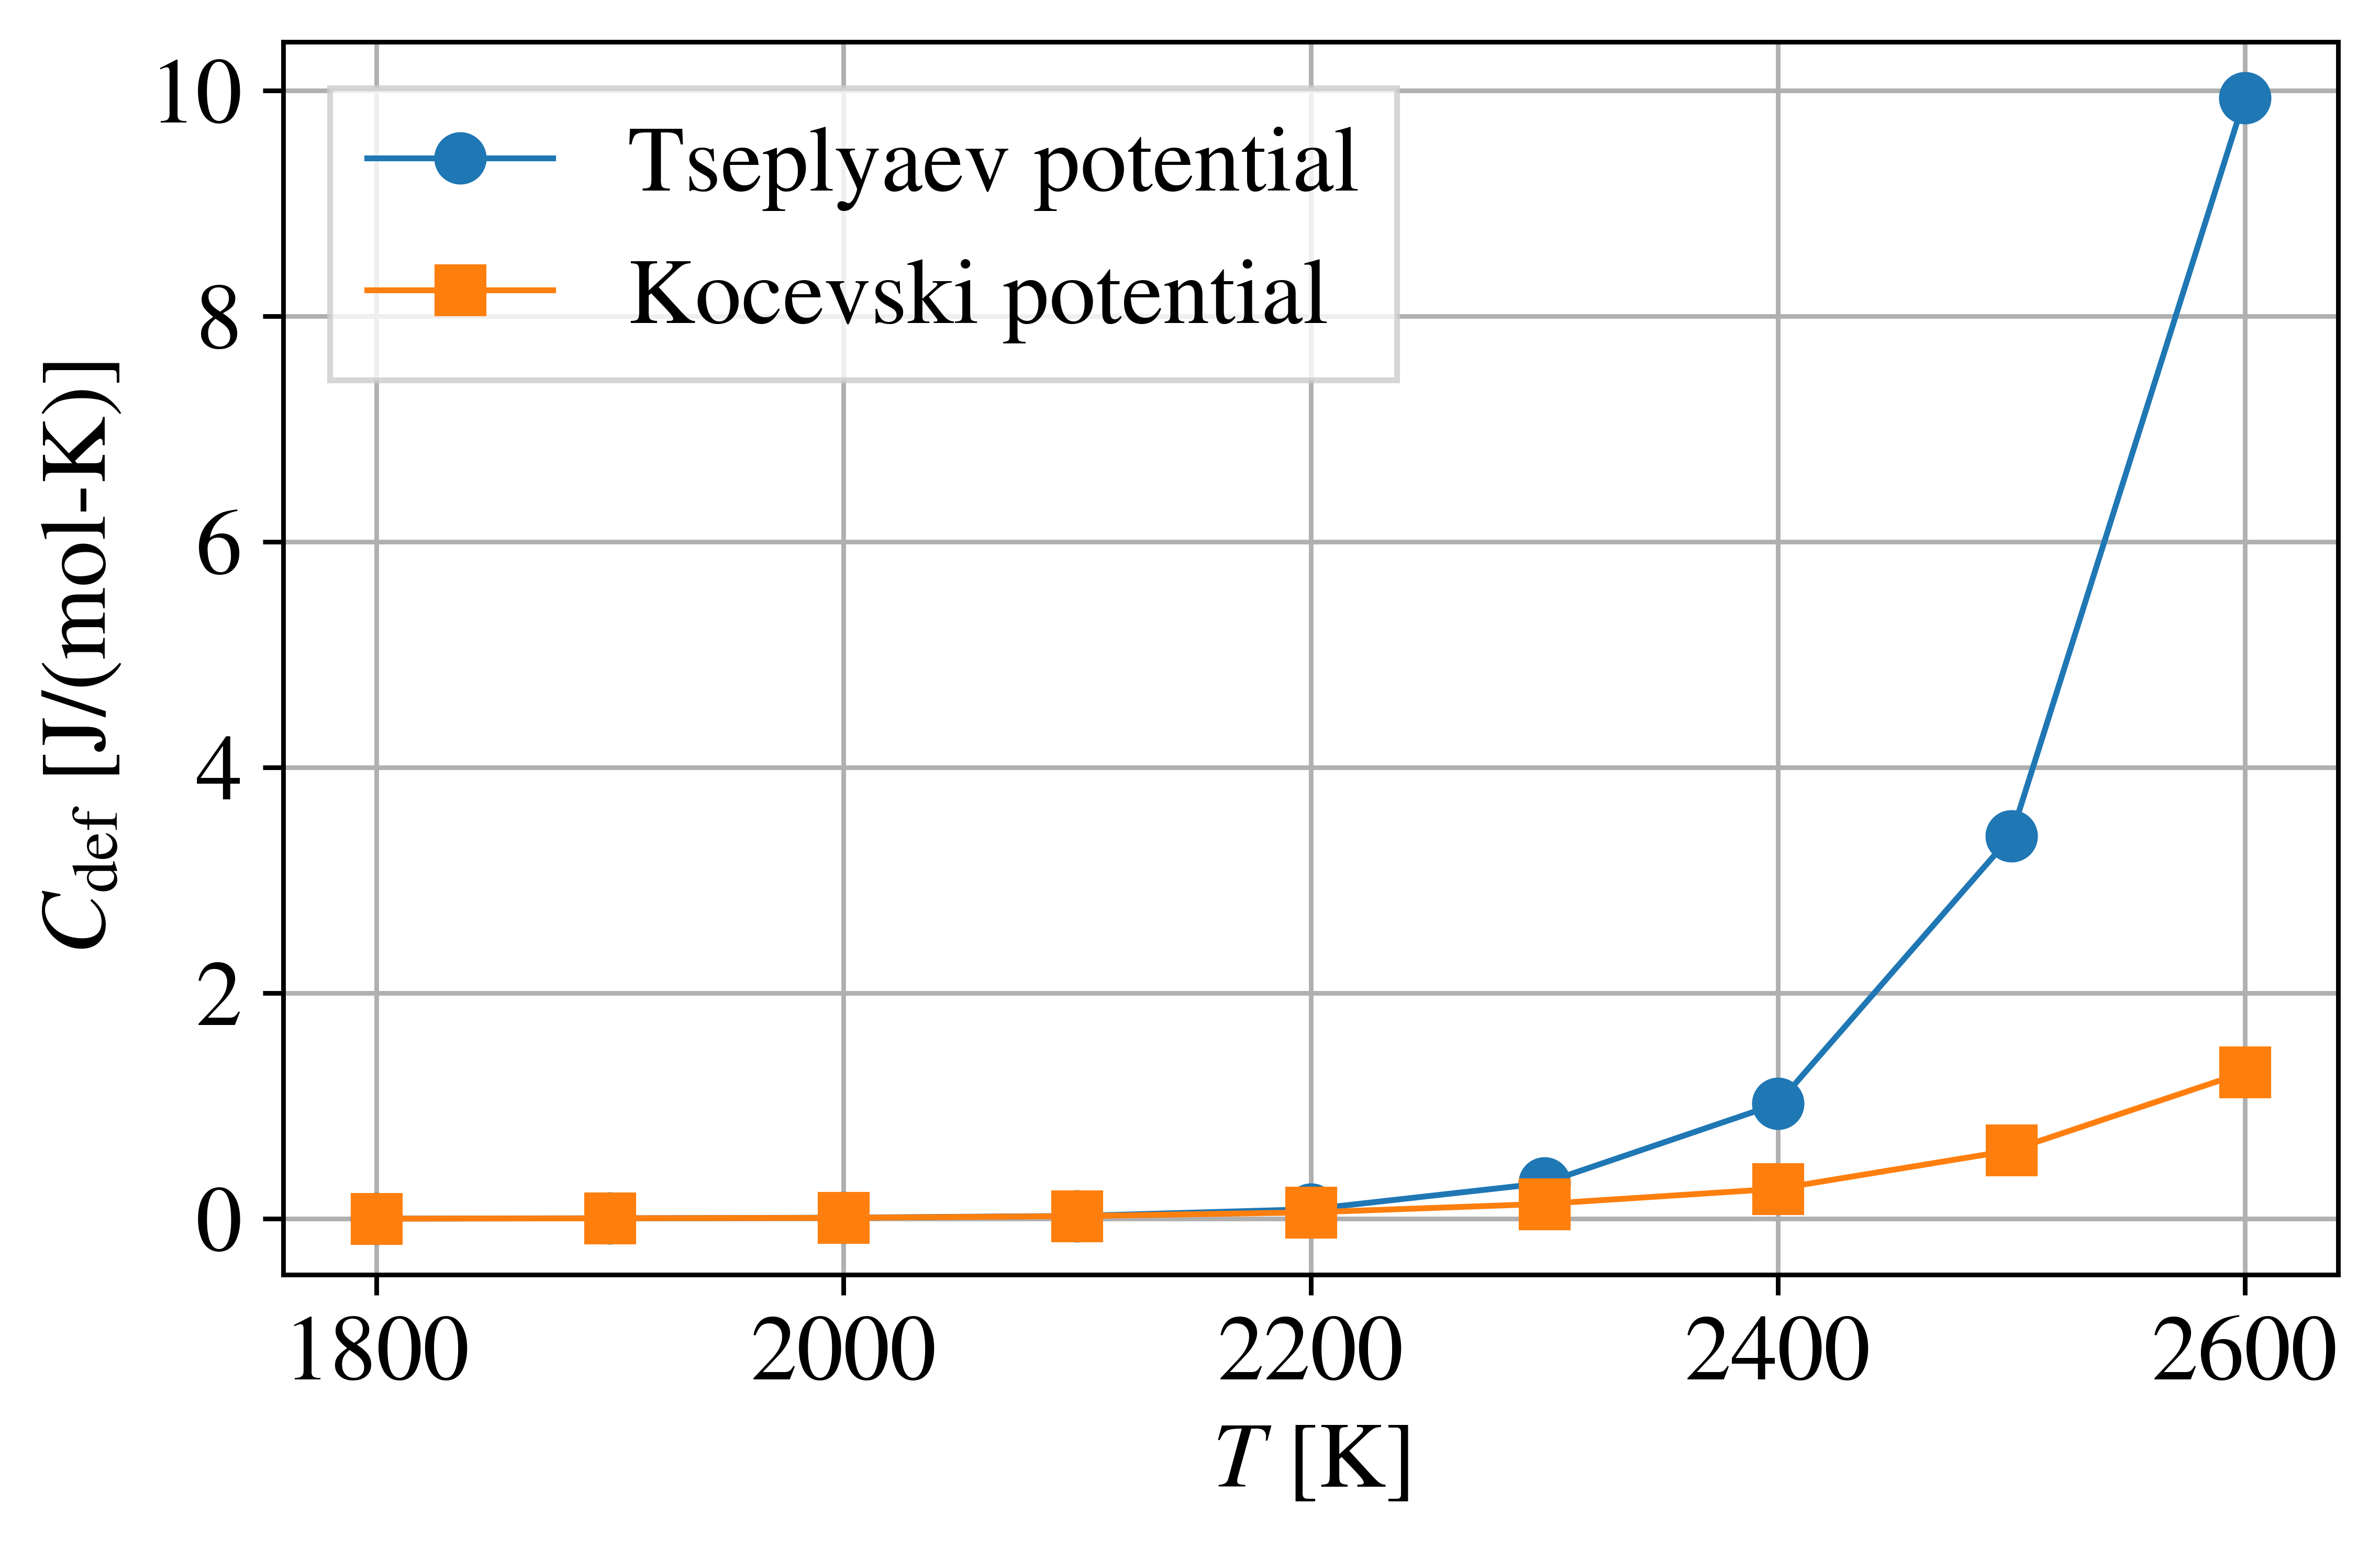
\includegraphics[width=0.5\textwidth]{C_def.png}
 \caption{Defect-induced heat-capacity contribution $C_{\mathrm{def}}(T)$ computed from Wigner-Seitz Frenkel-pair statistics using both the Tseplyaev and Kocevski interatomic potentials.}
 \label{Fig:C_def}
\end{figure*}

The resulting $C_{\mathrm{def}}(T)$ curves are shown in \cref{Fig:C_def}. For the Tseplyaev potential, $C_{\mathrm{def}}$ reaches $\sim$10~J/(mol-K) at 2600~K, whereas for the Kocevski potential it remains on the order of 1~J/(mol-K) at the same temperature. Thus, the order-of-magnitude difference in Frenkel-pair concentration between the two potentials translates into an order-of-magnitude difference in the defect contribution to the heat capacity. This might provide an explanation for why the Tseplyaev potential reproduces the strong curvature of the Hayes correlation, while the Kocevski potential yields a nearly linear $C_{P}(T)$: the latter underestimates the magnitude of the Frenkel-pair contribution and therefore fails to reproduce the superlinear component in $C_P(T)$.

A key observation is that the temperature range in which both the nitrogen diffusivity and Frenkel-pair concentration increase most rapidly (roughly 1800--2000~K) coincides with the onset of deviations from a purely phononic heat capacity in experiment and AIMD+DLM. This parallel behavior strongly suggests that UN undergoes a form of anion-sublattice disordering crossover at high temperature, qualitatively analogous to the oxygen superionic transition in UO$_2$.

% In the Tseplyaev potential description, nitrogen remains localized at low temperature, then progressively explores interstitial configurations, increasing both defect concentration and mobility and thereby enhancing $C_P(T)$.

Our results therefore support a defect-driven interpretation of the high-temperature heat capacity of UN: nitrogen Frenkel-pair formation and associated sublattice disorder provide a plausible intrinsic mechanism for the observed superlinear $C_P(T)$. The calculated $C_{\mathrm{def}}(T)$ should be regarded as qualitative, since the defect populations are sensitive to the choice of interatomic potential and \cref{Eq:C_def} is a simplified estimate. Nevertheless, the order-of-magnitude difference in Frenkel-pair concentration between the two potentials produces a correspondingly large difference in the defect contribution to the heat capacity. Thus, while the Tseplyaev potential predicts defect populations large enough to reproduce the curvature in the Hayes correlation and the Kocevski potential yields a much weaker response, the true intrinsic behavior of UN potentially lies between these limits.

This hypothesis is experimentally testable. High-purity UN samples with carefully controlled oxygen content, combined with high-temperature calorimetry and tracer-diffusion measurements, are therefore essential to determine whether an anion-mobility crossover and correlated superlinear enhancement in $C_P(T)$ occur near the temperatures predicted here.

\begin{acknowledgments}

The authors thank Jacob Eapen for the fruitful discussions and useful suggestions. This research made use of the resources of the High-Performance Computing Center at Idaho National Laboratory, which is supported by the Office of Nuclear Energy of the U.S. Department of Energy and the Nuclear Science User Facilities under Contract No. DE-AC07-05ID14517.

\end{acknowledgments}

\bibliography{apssamp} % Produces the bibliography via BibTeX.

\end{document}
